
\appendix
% 1. describe line is multi opacities, curves is single opacity.@xi Liu
% 2.1 ablation study: ori vs  adc vs live (SSIM, LPIPS, PSNR, training time)
% 2.2 loss ablation (delete loss sperately)
% 2.3 forward and backward time for different area curves resolution, and time statics of each forward module. backward time for different loss.
% 3.1 More examples for different paths @ chaoyi
% 3.3 More examples for different datasets (optional quantity) @ Xi and choose the demo for appendix @chaoyi 
% 3.3 training process of our LIVE
% 3.4 Shape analysis @Chaoyi
% 3.5 Our + LIVSS for DIV2K @Chaoyi
% 3.6 Convert our to XML SVG @Chaoyi

% 4. website
% 4.1 Changing teaser
% 4.2 Changing gallery
% 4.3 Updating comparison
% 4.4 Video of Training process Live and our
% 4.5 Updating Efficiency comparison
% 4.6 SVG link (Optional: Editting Based on LLIVS)

\section{Ablation Study}
% \begin{figure*}[!t]
% \centering
% \includegraphics[width=0.8\linewidth]{figures/ablations.pdf}
% \vspace{-1em}
% \caption{Ablation study on the proposed adaptive pruning and densification strategy and multi-opacity strategy. 
% }
% \vspace{-.5em}
% \label{fig:ablation}
% \end{figure*}

\label{sec:ablation}

\noindent\textbf{The effectiveness of adaptive pruning and densification and layer-wise vectorization strategy.}
We conduct an ablation study to evaluate the effectiveness of our adaptive pruning and densification strategy. Quantitative results are shown in Table~\ref{tab:adc_ablation_table}. To further investigate the flexibility of our framework, we incorporate a layer-wise curve addition strategy inspired by LIVE~\cite{xu2022live}, where curves are progressively added during training. Although this strategy achieves slightly better reconstruction metrics, it doubles the training time compared to our adaptive pruning and densification approach, making it less favorable for time-sensitive applications. Fig. \ref{fig:layerwise-training} shows our result with layer-wise image vectorization strategy.

\definecolor{bestrow}{RGB}{235,245,255}

\begin{table}[!h]
\centering
\caption{An ablation study on adaptive pruning and densification and layer-wise training strategy, evaluated on 512 closed curves with DIV2K dataset \cite{Timofte_2017_CVPR_Workshops}.}
% \vspace{-.5em}
\resizebox{0.7\linewidth}{!}{%
\begin{tabular}{l|cccc}
\hline
\textbf{Method} & $SSIM^\uparrow$ & $PSNR^\uparrow$ & $LPIPS^\downarrow$ & $Opt^\downarrow$ \\
\hline
No Strategy & 0.590 & 21.10 & 0.530 & \textbf{8.3 min} \\
% \rowcolor{bestrow}
~~-- w/ Prune\&Densify & 0.607 & 22.11 & 0.528 & 8.3 min \\
~~-- w/ Layer-wise & \textbf{0.613} & \textbf{22.21} & \textbf{0.521} & 16.2 min \\
\hline
\end{tabular}
}
\label{tab:adc_ablation_table}
\end{table}

\begin{figure*}[h]
\centering
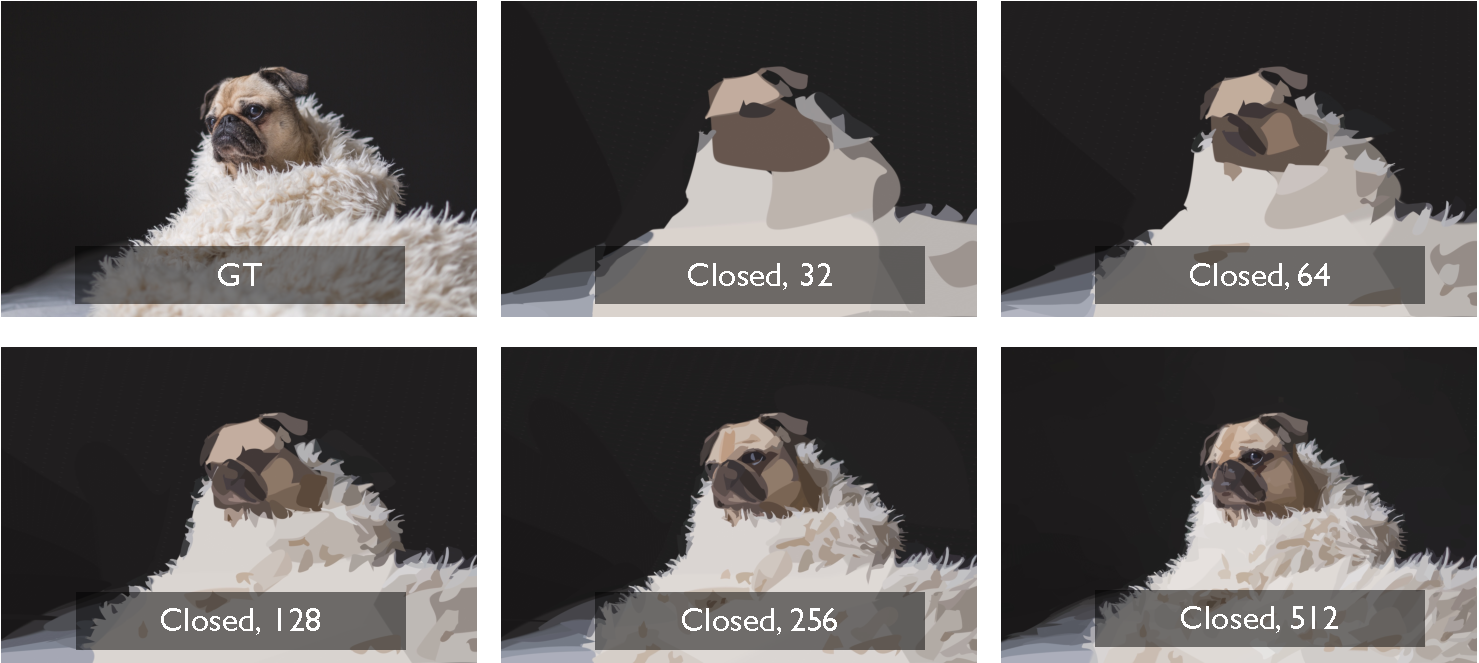
\includegraphics[width=0.9\linewidth]{figures/appendix_Layer-wised-training.pdf}
% \vspace{-2em}
\caption{Our Bézier Splatting is fully compatible with the layer-wise vectorization strategies \cite{xu2022live}. }
\label{fig:layerwise-training}
\end{figure*}

\noindent\textbf{Comparing different numbers of curves.} We progressively increase the number of curves for vectorizing a watercolor image (Fig. \ref{fig:curve number}) with numerous small spots. As the number of curves grows, our approach first reconstructs the foreground object, the bird, then gradually refines the smaller spots. This demonstrates that our method prioritizes the primary structure before optimizing finer details, effectively distributing curves to balance global structure and local texture representation, thanks to our adaptive pruning and densification strategy. 


\begin{figure}[h]
\centering
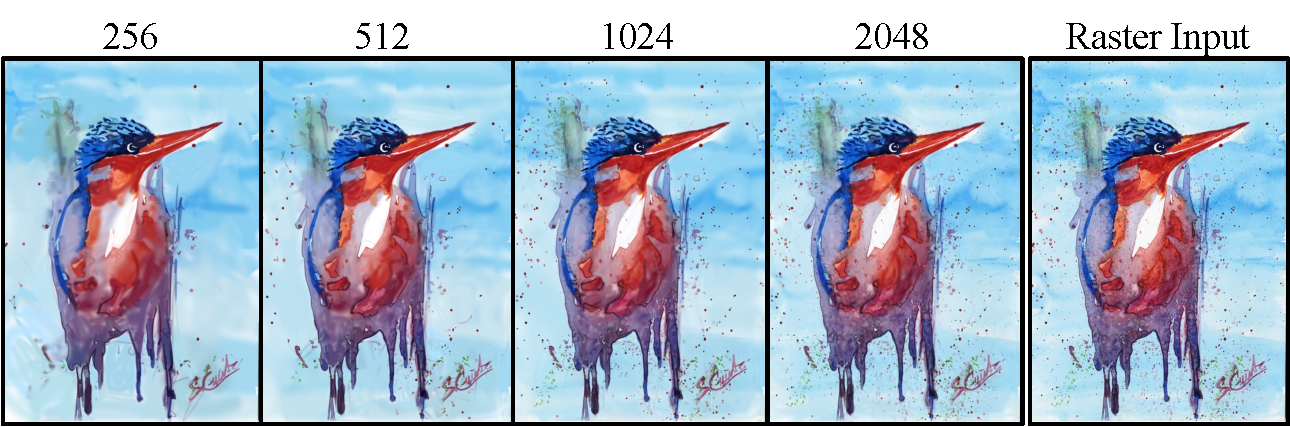
\includegraphics[width=0.9\linewidth]{figures/curve_number.pdf}
\vspace{-.5em}
\caption{A comparison of different curve numbers by Bézier Splatting. 
}
\label{fig:curve number}
\end{figure}



\noindent\textbf{A systematic evaluation of computation time.} To systematically evaluate the computational efficiency of our framework, we report detailed timing statistics across varying configurations of interpolation curve numbers and curve resolutions, as summarized in Table~\ref{tab:forward_backward_decomposed}. The total forward time includes two major parts: the Gaussian sampling and the Gaussian splatting. Increasing the number of interpolated curves within the closed Bézier curves leads to a near-linear growth in both forward and backward runtimes, demonstrating good computational scalability. When fixing the interpolation number (\textit{e.g.}, at 40) and varying the number of Bézier curves, the forward time increases moderately, reflecting the additional cost of handling finer spatial detail. The splatting stage dominates the forward time at higher number of curves due to the increased number of sampled points per region, while the Gaussian sampling time is the primary bottleneck at lower number of curves. This is attributed to overheads from sequential memory allocation and data transfer operations, which are not effectively parallelized on the GPU, suggesting potential for further optimization.

\begin{table}[!t]
\centering
\caption{A systematic evaluation of computation time. We test the forward and backward time (ms) under varying numbers of sampled curves within one closed Bézier curve (Inter. \#), and the total number of Bézier curves (Curve \#).}
\resizebox{1.0\linewidth}{!}{%
\begin{tabular}{ccccccc}
\toprule
\textbf{Inter. \#} & \textbf{Curve \#} & \textbf{Forward w/ gradient} & \textbf{Sample Gaussians} & \textbf{Splatting} & \textbf{Backward} & \textbf{Render (FPS)} \\
\midrule
20   & 2048 & 10.66 & 4.12   & 6.11   & 21.64 & 103.45 \\
40   & 2048 & 14.79 & 5.11   & 9.32   & 25.06 & 68.30  \\
80   & 2048 & 27.01 & 8.22   & 17.74  & 33.40 & 37.90  \\
\midrule
40   & 256  & 7.20  & 3.81 & 3.09  & 16.72 & 150.30 \\
40   & 512  & 7.70  & 3.88 & 3.67 & 17.42 & 144.30 \\
40   & 1024 & 10.39 & 4.06  & 5.96 & 19.96 & 114.30 \\
40   & 2048 & 14.79 & 5.11   & 9.32   & 25.06 & 68.30  \\
\bottomrule
\end{tabular}
}
\label{tab:forward_backward_decomposed}
\end{table}

\begin{table}[h]
\centering
\caption{A quantitative comparison between Adobe Image Trace \cite{illustrator2025} and our method across different images.}
\resizebox{1.0\linewidth}{!}{%
\begin{tabular}{c|cc|cc|cc|cc|cc}
\toprule
\textbf{Image ID} & \multicolumn{2}{c|}{0004} & \multicolumn{2}{c|}{0008} & \multicolumn{2}{c|}{0012} & \multicolumn{2}{c|}{0016} & \multicolumn{2}{c}{0020} \\
\midrule
\textbf{Method} & Adobe \cite{illustrator2025} & Ours & Adobe \cite{illustrator2025}& Ours & Adobe \cite{illustrator2025}& Ours & Adobe \cite{illustrator2025}& Ours & Adobe \cite{illustrator2025}& Ours \\
\midrule
\textbf{$SSIM^\uparrow$} & 0.835 & 0.849 & 0.645 & 0.637 & 0.658 & 0.658 & 0.627 & 0.628 & 0.814 & 0.822 \\
\textbf{$PSNR^\uparrow$} & 26.43 & 28.62 & 23.26 & 24.33 & 22.29 & 22.87 & 23.87 & 24.54 & 26.67 & 28.31 \\
\textbf{$LPIPS^\uparrow$} & 0.380 & 0.387 & 0.489 & 0.489 & 0.523 & 0.518 & 0.534 & 0.543 & 0.505 & 0.503 \\
\bottomrule
\end{tabular}
}
\label{tab:traditional_comparsion}
\end{table}


\noindent\textbf{Comparison with conventional image vectorization methods.}  We conduct a comparison against the Image Trace from Adobe Illustrator \cite{illustrator2025} on five images from the DIV2K dataset. Both methods are evaluated using the same number of parameters (around 20K). As shown in Table~\ref{tab:traditional_comparsion}, our method achieves higher fidelity, with an average PSNR of 25.734 db compared to 24.904 db of Image Trace.

\noindent\textbf{Arbitrary resolution rendering.}  
Our Bézier Splatting representation naturally supports rendering at arbitrary resolutions because all Gaussian parameters are analytically derived from the underlying Bézier curves. When higher-resolution images are required, proportionally increasing the sampling rate is sufficient to maintain reconstruction fidelity. For example, doubling the resolution simply doubles the sampling density. As shown in Table~\ref{tab:resolution}, rendering at higher resolutions (4K or 8K) with increased sampling preserves a comparable level of visual quality to the 2K baseline, without introducing noticeable artifacts. We report results on the first four images from the \cite{Timofte_2017_CVPR_Workshops} to illustrate this property.

\begin{table}[h]
\centering
\caption{
Results of Bézier Splatting rendered at different resolutions and sampling settings.  
Notation: ``orig.'' denotes the baseline sampling rate used during optimization, 
and ``$\times$S'' indicates S-times higher sampling density.
}
\label{tab:resolution}
% \vspace{0.3em}
\resizebox{0.6\linewidth}{!}{%
\begin{tabular}{lcccccc}
\toprule
\multirow{2}{*}{\textbf{Image ID}} & 
\multirow{2}{*}{\textbf{2K (orig.)}} &
\multicolumn{2}{c}{\textbf{4K}} & 
\multicolumn{2}{c}{\textbf{8K}} \\
\cmidrule(lr){3-4} \cmidrule(lr){5-6}
 &  & \textbf{orig.} & \textbf{($\times$2S)} & \textbf{orig.} & \textbf{($\times$4S)} \\
\midrule
0004 & 26.8976 & 27.1553 & 27.2761 & 25.9800 & 26.6594 \\
0008 & 21.2063 & 21.0614 & 21.4340 & 19.8318 & 21.1214 \\
0012 & 19.8816 & 19.9079 & 20.0900 & 18.9389 & 19.7760 \\
0016 & 22.3456 & 22.4327 & 22.5408 & 21.7088 & 22.3140 \\
\bottomrule
\end{tabular}
}
\end{table}

% \begin{table}[h]
% \centering
% \caption{Forward and backward time (ms) under different number of interplation curves  for 2048 closed curves.}
% \begin{tabular}{lccc}
% \toprule
% \textbf{Curve num} & \textbf{Forward Time (ms)} & \textbf{Backward Time (ms)} & \textbf{FPS} \\
% \midrule
% 20    & 10.66 (4.1, 6.1)                      & 21.64   &103.45                      \\
% 40  &14.79 (5.1, 9.3)                      & 25.06  & 68.3                         \\
% 80  & 27.01 (8.2, 17.7)                      & 33.4 & 37.9                     \\
% \bottomrule
% \end{tabular}
% \label{tab:forward_backward_resolution}
% \end{table}

% \begin{table}[h]
% \centering
% \caption{Forward and backward time (ms) under different curve resolutions with same interplation curves number: 40.}
% \begin{tabular}{lccc}
% \toprule
% \textbf{Curve Resolution} & \textbf{Forward Time (ms)} & \textbf{Backward Time (ms)} & \textbf{FPS}\\
% \midrule
% 256 curves    &7.2 (3.807, 3.09)                       & 16.724        & 150.3       \\
% 512 curves   &7.7 (3.877, 3.669)                       & 17.424        & 144.3        \\
% 1024 curves  &10.39 (4.06, 5.958)                       & 19.96        & 114.3        \\
% 2048 curves  &14.79 (5.1, 9.3)                      & 25.06  & 68.3                         \\
% \bottomrule
% \end{tabular}
% \label{tab:forward_backward_resolution}
% \end{table}

\section{Details of Adaptive Pruning and Densification}
To provide a clearer understanding of our optimization behavior, we present here the detailed procedure of the pruning–densification algorithm \ref{alg:adaptive_pruning_densification} used in our Bézier-splatting framework.This algorithm is designed to mitigate the local-minima issue observed in 3D Gaussian Splatting (3DGS) and is adapted in our Bézier-splatting framework, where suboptimal primitive initialization leaves certain regions insufficiently covered.
Inspired by the pruning–splitting mechanism of 3DGS [1], our method dynamically reallocates Bézier curves according to the reconstruction error map: curves with low opacity, small area, or high overlap with nearby curves of similar color are pruned, while new curves are inserted into regions with high reconstruction error to improve coverage.
This reallocation keeps the total curve budget fixed, enhances reconstruction quality, and helps the optimization escape poor local minima.
For open curves, we additionally introduce a splitting rule:
if the middle opacity of a curve is more than 0.5 lower than that of both endpoints, the curve is split into two segments to better adapt to local structure variations.


\begin{algorithm}[t]
\caption{\textbf{Adaptive Pruning and Densification for Closed Bézier Curves}}
\label{alg:adaptive_pruning_densification}
\begin{algorithmic} % no [1] => no line numbers

% ---- line between caption and Notation ----

% ---- Notation (operators in bold), one per line ----
\STATE \textbf{Notation:}
\STATE \quad $\mathbf{opacity}(b)$ — mean opacity of curve $b$.
\STATE \quad $\mathbf{area}(b)$ — area enclosed by curve $b$.
\STATE \quad $\mathbf{colordiff}(b_i,b_j)$ — Euclidean color difference between curves $b_i$ and $b_j$.
\STATE \quad $\mathbf{IoU}(b_i)$ — intersection-over-union between the bounding box of $b_i$ and neighboring curves with $\mathbf{colordiff}<0.03$.
\STATE \quad $\mathbf{ConnectedComponents}(E)$ — connected error regions extracted from the quantized error map.

% ---- line below Notation ----
\STATE {\rule{\linewidth}{0.5pt}}


% ---- Inputs / Outputs ----
\STATE \textbf{Input}~: Closed Bézier curve set $\mathcal{B}=\{b_1,\dots,b_N\}$; opacity map $\alpha$; error map $E$; iteration index $t$.
\STATE \textbf{Output}: Updated curve set $\mathcal{B}'$.



% ---- Algorithm body ----
\STATE Initialize $\mathcal{B}' \leftarrow \mathcal{B}$.

\STATE \textbf{Pruning phase}
\FOR{$i \gets 1$ \TO $N$}
  \IF{$\mathbf{opacity}(b_i) < \tau_{\mathbf{opacity}}(t)$}
    \STATE Remove $b_i$ from $\mathcal{B}'$. \COMMENT{Low-opacity pruning}
  \ENDIF
  \IF{$\mathbf{area}(b_i) < \tau_{\mathbf{area}}$}
    \STATE Remove $b_i$ from $\mathcal{B}'$. \COMMENT{Small-area pruning}
  \ENDIF
  \IF{$\mathbf{IoU}\!\big(b_i, \{\,b_j \in \mathcal{B} \mid \mathbf{colordiff}(b_i,b_j) < 0.03\,\}\big) > 0.9$}
    \STATE Remove $b_i$ from $\mathcal{B}'$. \COMMENT{Redundant-overlap pruning}
  \ENDIF
\ENDFOR

\STATE \textbf{Densification phase}
\STATE $\mathcal{R} \leftarrow \mathbf{ConnectedComponents}(E)$.
\STATE $\mathcal{R}_{\mathbf{sorted}} \leftarrow \mathbf{SortByArea}(\mathcal{R})$.
\FOR{each region $r_j \in \mathcal{R}_{\mathbf{sorted}}$}
  \IF{curve budget allows}
    \STATE Insert a new closed Bézier curve into $r_j$.
  \ENDIF
\ENDFOR

\STATE \textbf{return} $\mathcal{B}'$.
\end{algorithmic}
\end{algorithm}



% \clearpage

\section{Convert Bézier Splatting to Standard SVG Format}


As described in Algorithm~\ref{alg:svg-export}, we convert our optimized Bézier Splatting representation into a standard SVG file for compatibility with downstream vector editing tools.
Each curve is represented by a set of $3k + 1$ control points $\mathcal{C}_i \in \mathbb{R}^{(3k+1) \times 2}$, corresponding to $k$ continuous cubic Bézier segments.
These control points are normalized to the range $[-1, 1]$ and are first transformed into pixel coordinates according to the canvas size $(W, H)$.

For each curve $i$, we initialize the SVG path string $d$ with a \texttt{[M $P_i^0$]} command.
We then iteratively construct each cubic segment using three internal control points:
$(p_1, p_2, p_3) = (P_i^{3j+1}, P_i^{3j+2}, P_i^{3j+3})$,
and append the segment as a path command \texttt{[C $p_1$, $p_2$, $p_3$]} to $d$.
After all segments are processed, a \texttt{[Z]} is appended to close the path.

Each path $d$ is then associated with a fill color $(r, g, b)$, computed via sigmoid activation on the optimized feature vector $\mathcal{F}_i$, and opacity 1.0.
The result is stored in a global path set $\mathcal{S}$, and all paths are assembled into the final SVG file $S$.
This output is directly compatible with standard vector graphics tools such as Adobe Illustrator.

\begin{algorithm}[!h]
   \caption{\textbf{Convert Bézier Splatting to Standard SVG}}
   \label{alg:svg-export}
\begin{algorithmic}
   \STATE {\bfseries Input:} Optimized control points $\mathcal{C} \in \mathbb{R}^{N \times (3k+1) \times 2}$, feature colors $\mathcal{F} \in \mathbb{R}^{N \times 3}$, canvas size $(W, H)$
   \STATE {\bfseries Output:} SVG file $S$ containing cubic Bézier paths \\
   \FOR{each curve $i = 1$ to $N$}
   \STATE $P_i \leftarrow \frac{\mathcal{C}_i + 1}{2} \cdot (W, H)$
    \STATE $(r, g, b) \leftarrow \text{sigmoid}(\mathcal{F}_i) \times 255$
    \STATE Initialize path $d \leftarrow \texttt{[M $P_i^0$]}$

    \FOR{each segment $j = 1$ to $k$} 
    \STATE $(p_1, p_2, p_3) \leftarrow $($P_i^{3j + 1}, P_i^{3j + 2}, P_i^{3j + 3})$\;
    \STATE $d \oplus \texttt{[C $p_1$, $p_2$, $p_3$]}$ \\
    \ENDFOR
    \STATE $d \oplus \texttt{Z}$\;
    \STATE $\mathcal{S} \leftarrow \mathcal{S} \cup \{ \text{path}(d,\, \text{fill} = (r, g, b),\, \text{opacity} = 1.0) \}$
    \ENDFOR
   \STATE {\bfseries Return:} SVG file assembled from all paths
\end{algorithmic}
\end{algorithm}

\section{Bézier Splatting Supports Flexible Curve Attributes}
All 2D Gaussians in our method are generated via a differentiable sampling algorithm, which makes it straightforward to incorporate user-defined shape attributes, such as linear-gradient fills in color or opacity. To demonstrate the extensibility of our model, we evaluate the multi-opacity scheme for open curves: each Bézier segment within an open curve is assigned an independent opacity value. This design enables users to either maintain consistent sampling point appearance across segments or apply customized interpolation strategies. This strategy significantly improves vectorization quality for open curves, as shown in Table ~\ref{tab:ablation_table}. Since closed curves are the primary representation format in SVG, we adopt a uniform setting for opacity and color in those regions to ensure a full compatibility with existing vector graphic tools. Nonetheless, users can still follow the above multi-opacity scheme to implement linear-gradient fills for both opacity and color, enhancing the flexibility and expressiveness of vector graphics.

\begin{table}[!h]
\centering
\caption{An ablation study on the number of opacity parameters per curve, evaluated on 512 open curves with DIV2K dataset \cite{Timofte_2017_CVPR_Workshops}.}
\vspace{-.5em}
\resizebox{0.45\linewidth}{!}{%
\begin{tabular}{l|ccc}
\hline
  \textbf{Method}  & $SSIM^\uparrow$   & $PSNR^\uparrow$    & $LPIPS^\downarrow$   \\ 
  \hline
  % Full (w/ Prune\&Densify, 3-opacity)  &\textbf{0.65}  &\textbf{23.79}   &\textbf{0.50}  \\
    3-opacity  &\textbf{0.65}  &\textbf{23.79}   &\textbf{0.50}  \\
    % ~~- w/o Prune\&Densify   & 0.63   & 23.23   & \textbf{0.50}   \\
   1-opacity   &0.63    &22.97   &0.51    \\
  % & \checkmark  & 3  &   &  &   \\
  \hline

\end{tabular}
}
\label{tab:ablation_table}
\end{table}










\section{More Comparisons}




% We evaluate the differentiable VG methods on more natural images. We quantitatively evaluate our method on another natural image dataset, Kodak \cite{kodak1999}, and the results are shown in Table \ref{tab:comparisons_kodak} and Fig. \ref{fig:appendix_Kodak}.
% Fig. \ref{fig:app_comparsion_0}, \ref{fig:app_comparsion_1}, \ref{fig:app_comparsion_2}, \ref{fig:app_comparsion_3}, and \ref{fig:app_comparsion_4} show more qualitative comparisons. In the second image, our method successfully captures finer details in the blanket, preserving intricate textures and subtle variations that are less accurately represented by other methods. This demonstrates the superior representation capacity of our Bézier Splatting, particularly for complex textures and high-frequency details while maintaining structural integrity. 

We present more qualitative comparisons on the DIV2K~\cite{Timofte_2017_CVPR_Workshops} dataset. As shown in Fig.~\ref{fig:app_comparsion_0}, Fig.~\ref{fig:app_comparsion_1}, Fig.~\ref{fig:app_comparsion_2}, Fig.~\ref{fig:app_comparsion_3}, and Fig.~\ref{fig:app_comparsion_4}, our method shows consistent improvements over the baselines, including better preservation of fine details, higher rendering fidelity, fewer visual artifacts, and more accurate geometric structures. Furthermore, as the number of curves increases, our method demonstrates a significantly improved representational ability, enabling more precise reconstruction of complex shapes, and fine-grained structures.

We further evaluate our method on another natural image dataset, Kodak~\cite{kodak1999}. Due to the slow vectorization speed of LIVE \cite{xu2022live}, we compare with DiffVG on open curves only. As shown in Table~\ref{tab:comparisons_kodak}, our method consistently outperforms DiffVG across quantitative metrics including PSNR, SSIM, and LPIPS. 
% Furthermore, the qualitative results presented in Fig.~\ref{fig:appendix_Kodak} demonstrate that our method produces high visual fidelity, clean structures, sharp details, even in regions with complex textures.

% \begin{table*}[!h]
%     \centering
    
%     \caption{
%          A quantitative evaluation on the Kodak dataset \cite{kodak1999} (256 to 2,048 open curves).
%     }
%     % \vspace{-1em}
%     \resizebox{1\textwidth}{!}{
%         \begin{tabular}{l|ccc|ccc|ccc|ccc}
%             \toprule
%              \multirow{2}{*} {\textbf{Method} 
%              % / \textbf{Curve \#} 
%              } & \multicolumn{3}{c|}{\textbf{256}} & \multicolumn{3}{c|}{\textbf{512}} & \multicolumn{3}{c|}{\textbf{1024}} & \multicolumn{3}{c}{\textbf{2048}} \\
                        
%              & $SSIM^\uparrow$   & $PSNR^\uparrow$    & $LPIPS^\downarrow$ & $SSIM^\uparrow$   & $PSNR^\uparrow$    & $LPIPS^\downarrow$ & $SSIM^\uparrow$   & $PSNR^\uparrow$    & $LPIPS^\downarrow$ & $SSIM^\uparrow$   & $PSNR^\uparrow$    & $LPIPS^\downarrow$   \\
%             \hline
            
%             \multirow{2}{*}{Open} 
%              DiffVG & 0.601 & 23.43 & 0.535  & 0.645 & 24.70 & 0.495  & 0.699 & 26.04 & 0.439  & 0.762 & 27.56 & 0.360  \\
%             Ours & \textbf{0.679} & \textbf{26.18} & \textbf{0.457}  & \textbf{0.743} & \textbf{27.90} & \textbf{0.383}  & \textbf{0.797} & \textbf{29.24} & \textbf{0.310}  & \textbf{0.793} & \textbf{28.75} & \textbf{0.300}  \\
            
%             \hline
%             \multirow{3}{*}{Closed} 
%             & DiffVG & 0.622 & 24.11 & 0.513  & 0.666 & 25.34 & 0.475  & 0.719 & 26.66 & 0.420  & 0.779 & 28.17 & 0.350  \\
%             & LIVE  & \textbf{0.647} & \textbf{24.61} & \textbf{0.495}  & \textbf{0.693} & \textbf{26.00} & \textbf{0.447}  & \textbf{0.742} & \textbf{27.47} & \textbf{0.392} & - & - & -  \\
%             & \textbf{Bézier splatting (Ours)} & 0.625 & 24.37 & 0.510  & 0.667 & 25.30 & 0.471   & 0.713 & 26.69 & 0.423  & \textbf{0.757} & \textbf{27.66} & \textbf{0.372}  \\

%             \hline
%         \end{tabular}
%     }
%     \label{tab:comparisons_kodak}
% \end{table*}

\begin{table*}[!h]
    \centering
    \caption{
        A quantitative evaluation on the Kodak dataset~\cite{kodak1999} with 256 to 1024 curves. 
        We report results on open curves.
        % using SSIM, PSNR (higher is better), and LPIPS (lower is better).
    }
    \resizebox{1\textwidth}{!}{
        \begin{tabular}{l|l|ccc|ccc|ccc}
            \toprule
            \multirow{2}{*} & \multirow{2}{*}{\textbf{Method}} 
             & \multicolumn{3}{c|}{\textbf{256}} 
             & \multicolumn{3}{c|}{\textbf{512}} 
             & \multicolumn{3}{c}{\textbf{1024}} 
              \\
             
             & & $SSIM^\uparrow$ & $PSNR^\uparrow$ & $LPIPS^\downarrow$
               & $SSIM^\uparrow$ & $PSNR^\uparrow$ & $LPIPS^\downarrow$
               & $SSIM^\uparrow$ & $PSNR^\uparrow$ & $LPIPS^\downarrow$ \\
            \midrule

            \multirow{2}{*}{Open} 
            & DiffVG & 0.601 & 23.43 & 0.535  
                    & 0.645 & 24.70 & 0.495  
                    & 0.699 & 26.04 & 0.439   \\
            & Ours   & \textbf{0.679} & \textbf{26.18} & \textbf{0.457}  
                    & \textbf{0.743} & \textbf{27.90} & \textbf{0.383}  
                    & \textbf{0.797} & \textbf{29.24} & \textbf{0.310}  \\

            \midrule
            \multirow{2}{*}{Closed} 
            & DiffVG & \textbf{0.622} & 24.11 & \textbf{0.513}  
                    & \textbf{0.666} & 25.34 & 0.475  
                    & \textbf{0.719} & 26.66 & \textbf{0.420}  \\
            % & LIVE   & \textbf{0.647} & \textbf{24.61} & \textbf{0.495}  
            %         & \textbf{0.693} & \textbf{26.00} & \textbf{0.447}  
            %         & \textbf{0.742} & \textbf{27.47} & \textbf{0.392}  
            %         & - & - & - \\
            & Ours 
                    & 0.621 & \textbf{24.19} & 0.519 
                    & 0.664 & \textbf{25.61} &0.485 
                    & 0.708 & \textbf{26.91} & 0.448  \\
            % % \multirow{3}{*}{Closed} 
            % & DiffVG & 0.622 & 24.11 & 0.513  
            %         & 0.666 & 25.34 & 0.475  
            %         & 0.719 & 26.66 & 0.420  
            %         & 0.779 & 28.17 & 0.350 \\
            % % & LIVE   & \textbf{0.647} & \textbf{24.61} & \textbf{0.495}  
            % %         & \textbf{0.693} & \textbf{26.00} & \textbf{0.447}  
            % %         & \textbf{0.742} & \textbf{27.47} & \textbf{0.392}  
            % %         & - & - & - \\
            % & Ours 
            %         & 0.621 & 24.19 & 0.519 
            %         & 0.664 & 25.61 &0.485 
            %         & 0.708 & 26.91 & 0.448  
            %         & \textbf{0.755} & \textbf{28.02} & \textbf{0.393} \\
            \bottomrule
        \end{tabular}
    }
    \label{tab:comparisons_kodak}
\end{table*}





\section{More Image Vectorization Results}
% We sho our method on more image examples across a broader range of image domains.
% Fig. \ref{fig:appendix_large_line} shows more natural image examples by open curves, while Fig. \ref{fig:appendix_large_closed} shows more results by closed curves.
Fig. \ref{fig:appendix_large_div}, Fig. \ref{fig:appendix_Kodak}, and Fig. \ref{fig:appendix_large_animation} show more results on natural images from DIV2K \cite{Timofte_2017_CVPR_Workshops} and Kodak \cite{kodak1999}, as well as animation images from DanbooRegion \cite{DanbooRegion2020}, respectively. The results demonstrate that both the global structure and local texture of the images are well reconstructed, highlighting the effectiveness of our approach in capturing fine details and complex shapes. 





\begin{figure*}[t]
\centering
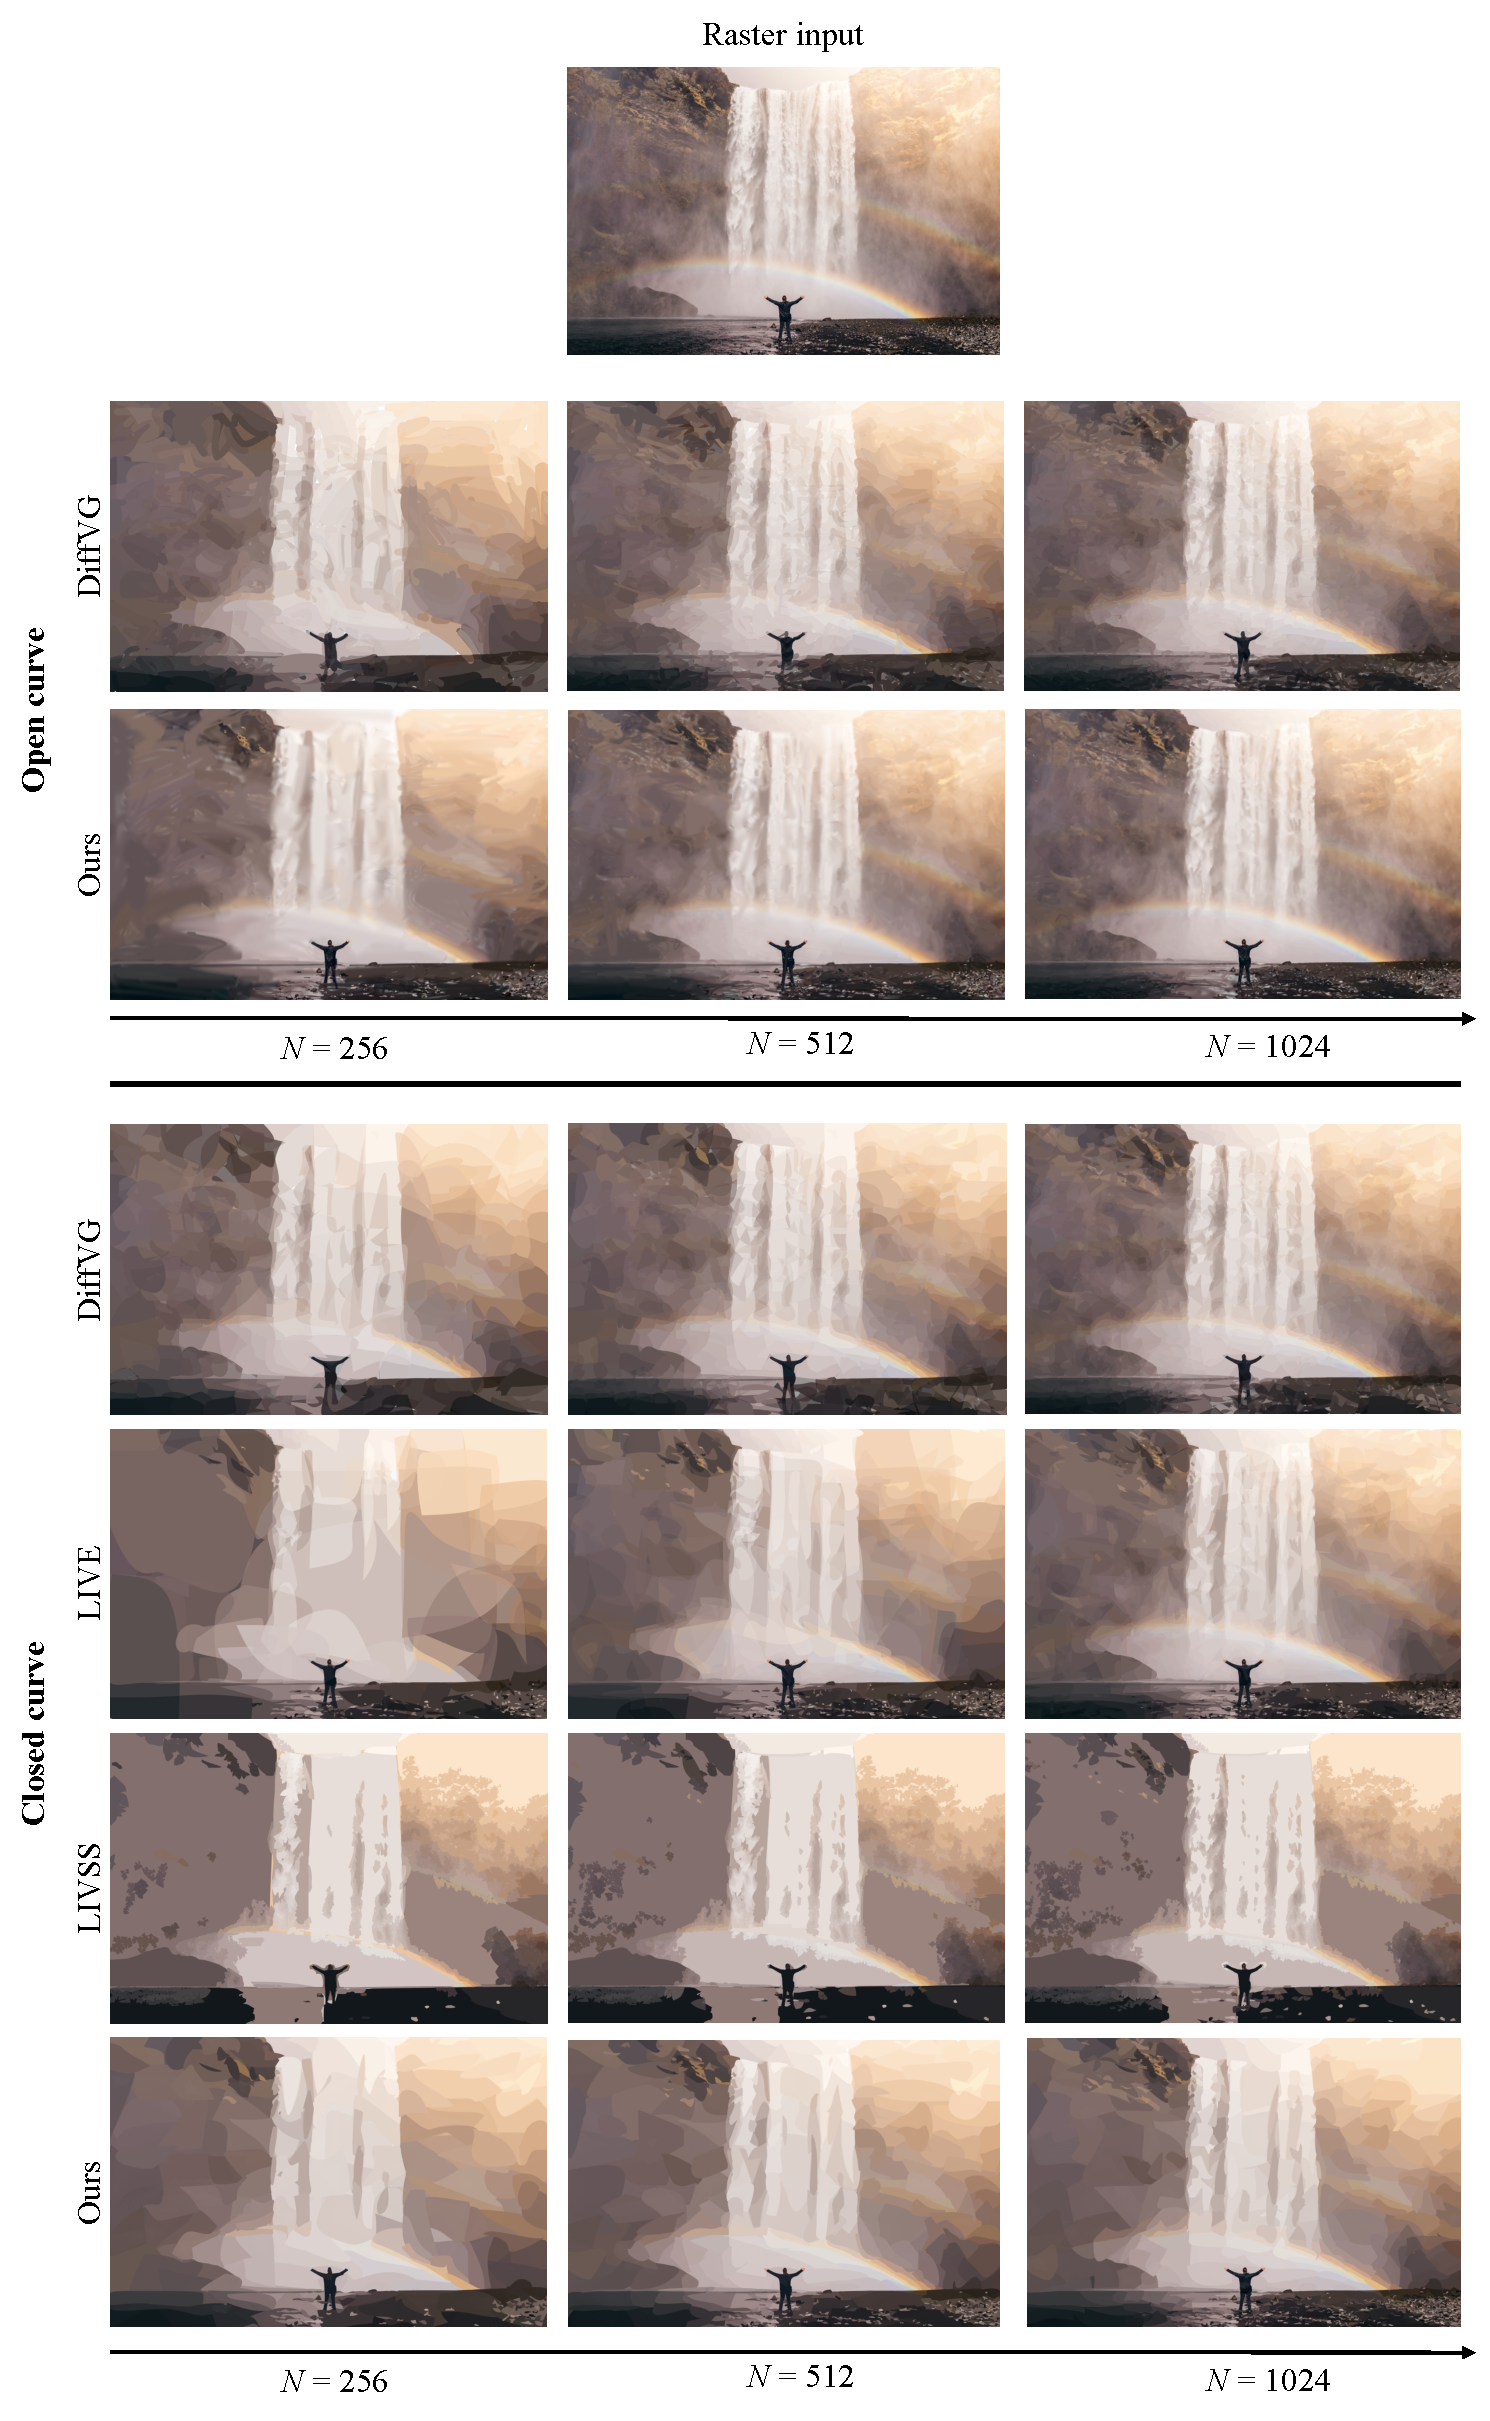
\includegraphics[width=1.0\linewidth]{figures/app_comparsion_0.pdf}
% \vspace{-2em}
\caption{A qualitative comparison of our method and the existing differentiable VG rasterization method on DIV2K dataset \cite{Timofte_2017_CVPR_Workshops}.
}
\label{fig:app_comparsion_0}
\end{figure*}

\begin{figure*}[t]
\centering
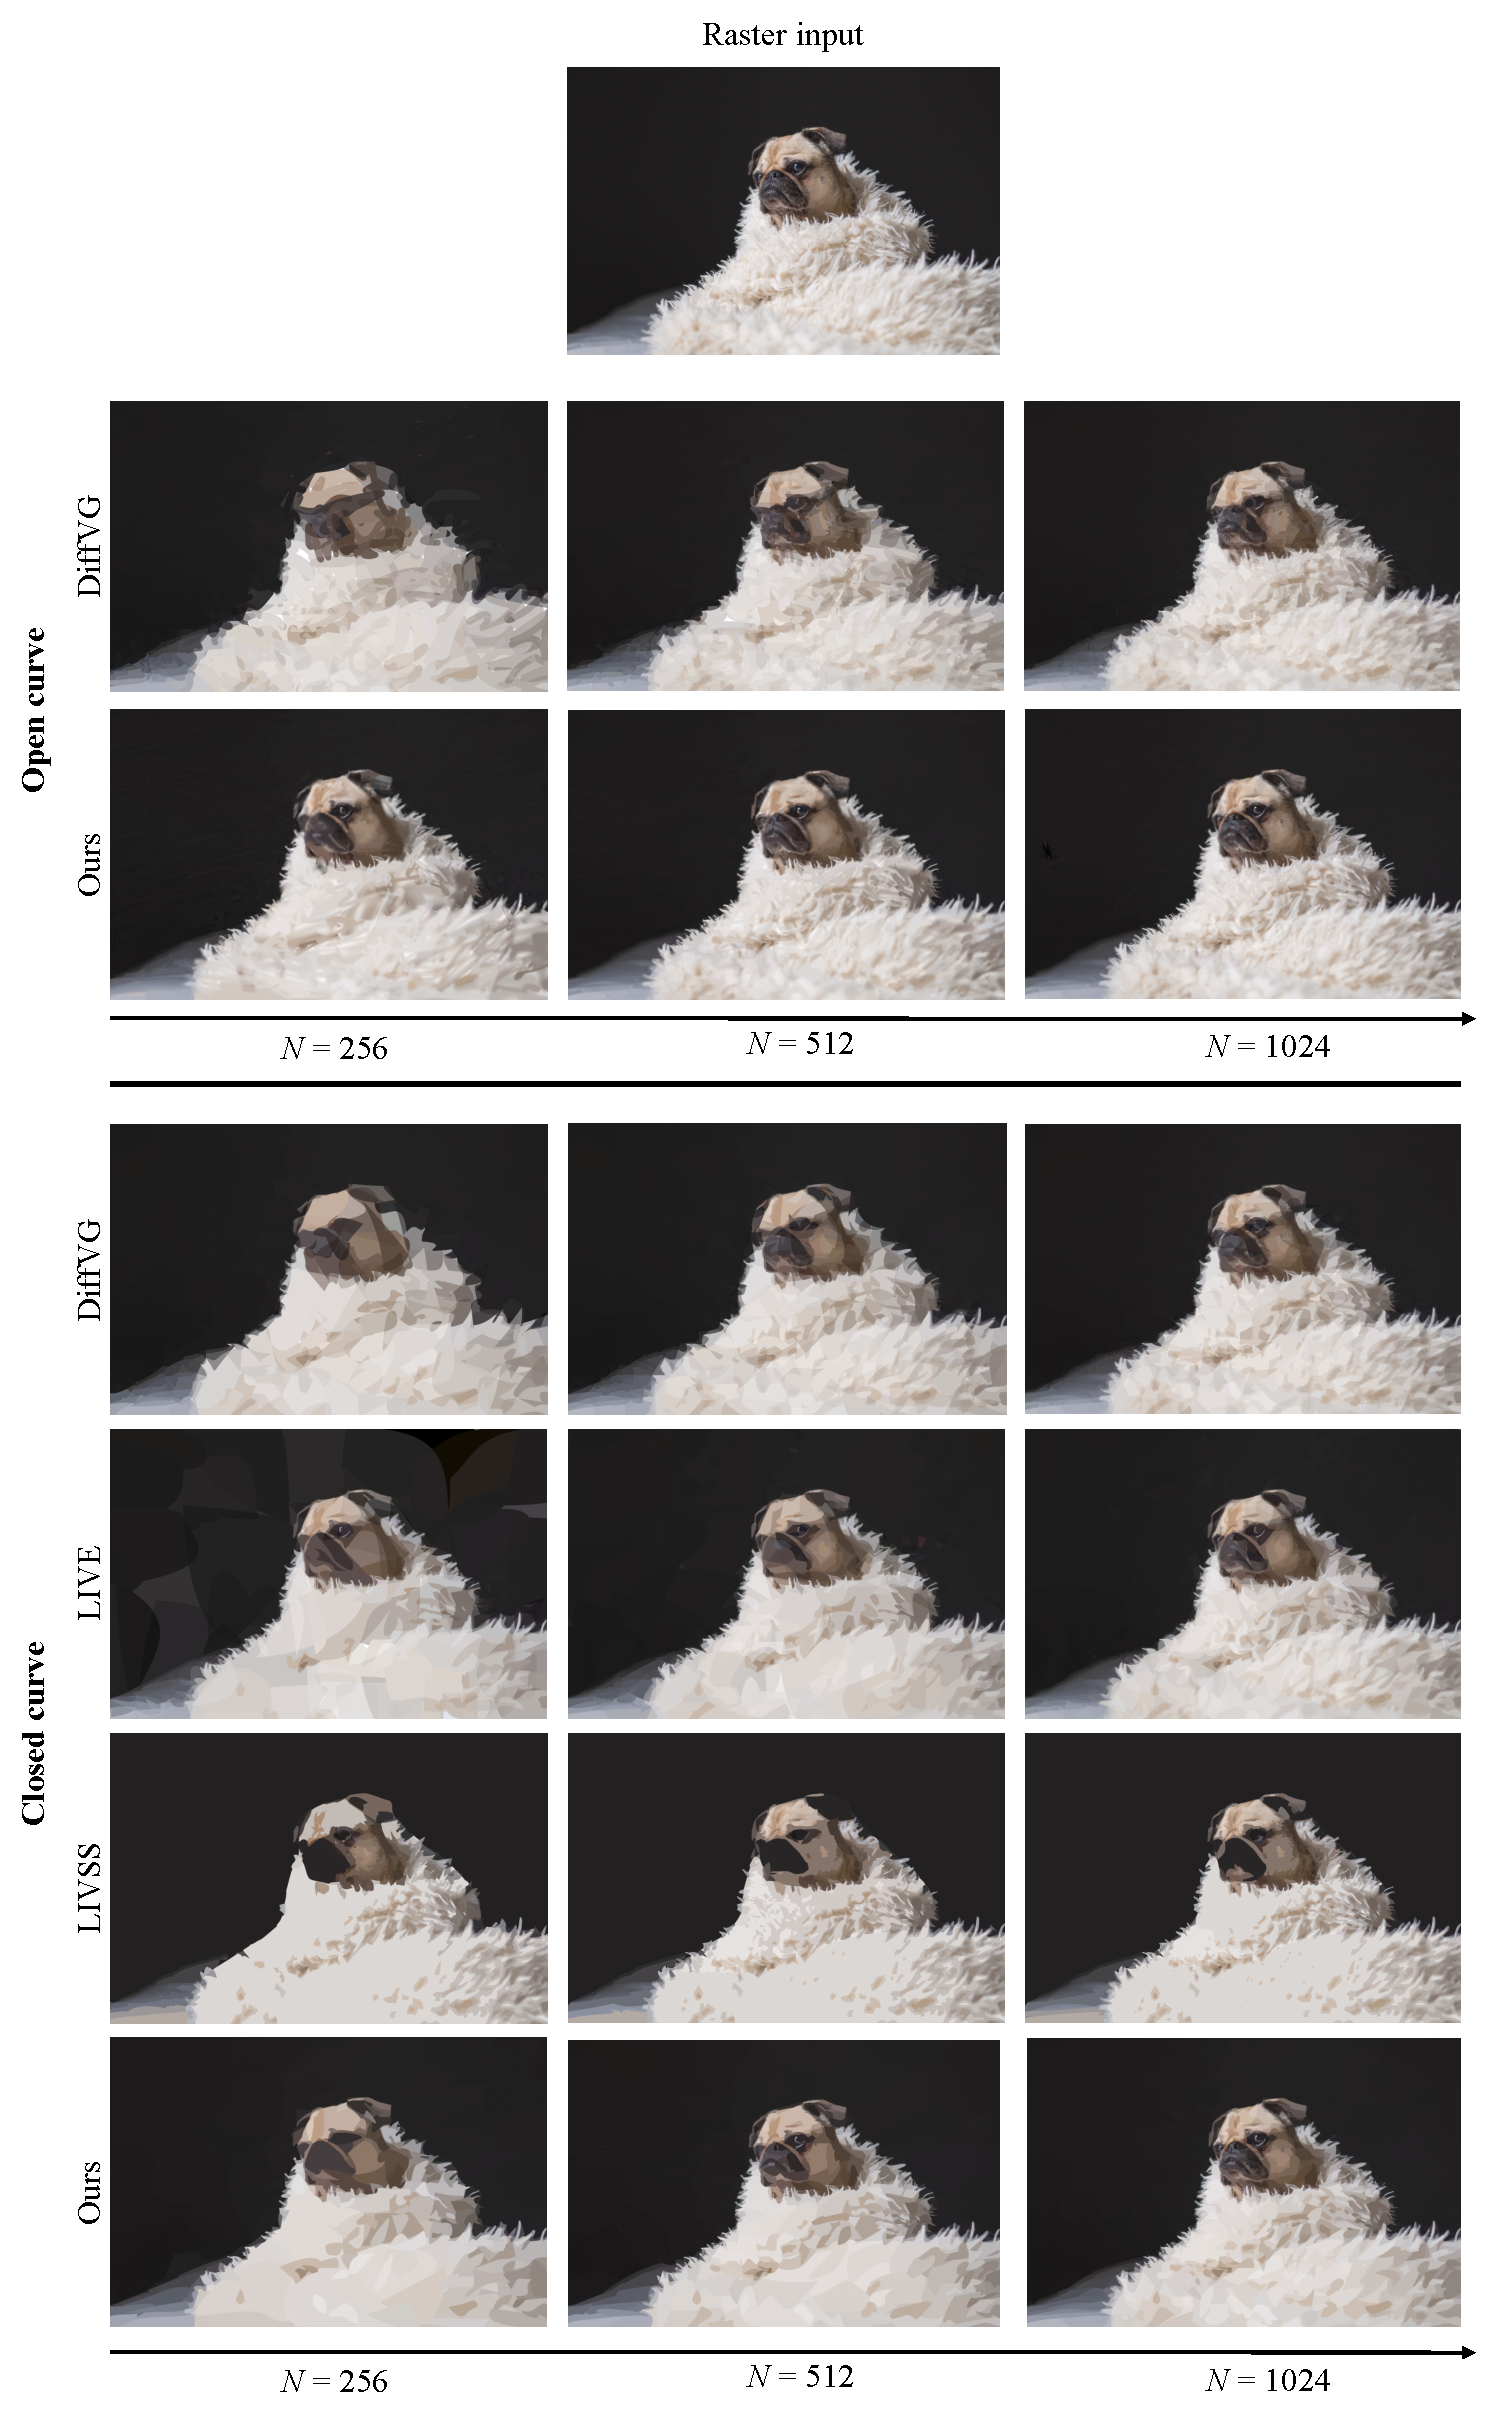
\includegraphics[width=1\linewidth]{figures/app_comparsion_1.pdf}
% \vspace{-2em}
\caption{More qualitative comparisons of our method and the existing differentiable VG rasterization method on DIV2K dataset \cite{Timofte_2017_CVPR_Workshops}.
}
\label{fig:app_comparsion_1}
\end{figure*}

\begin{figure*}[t]
\centering
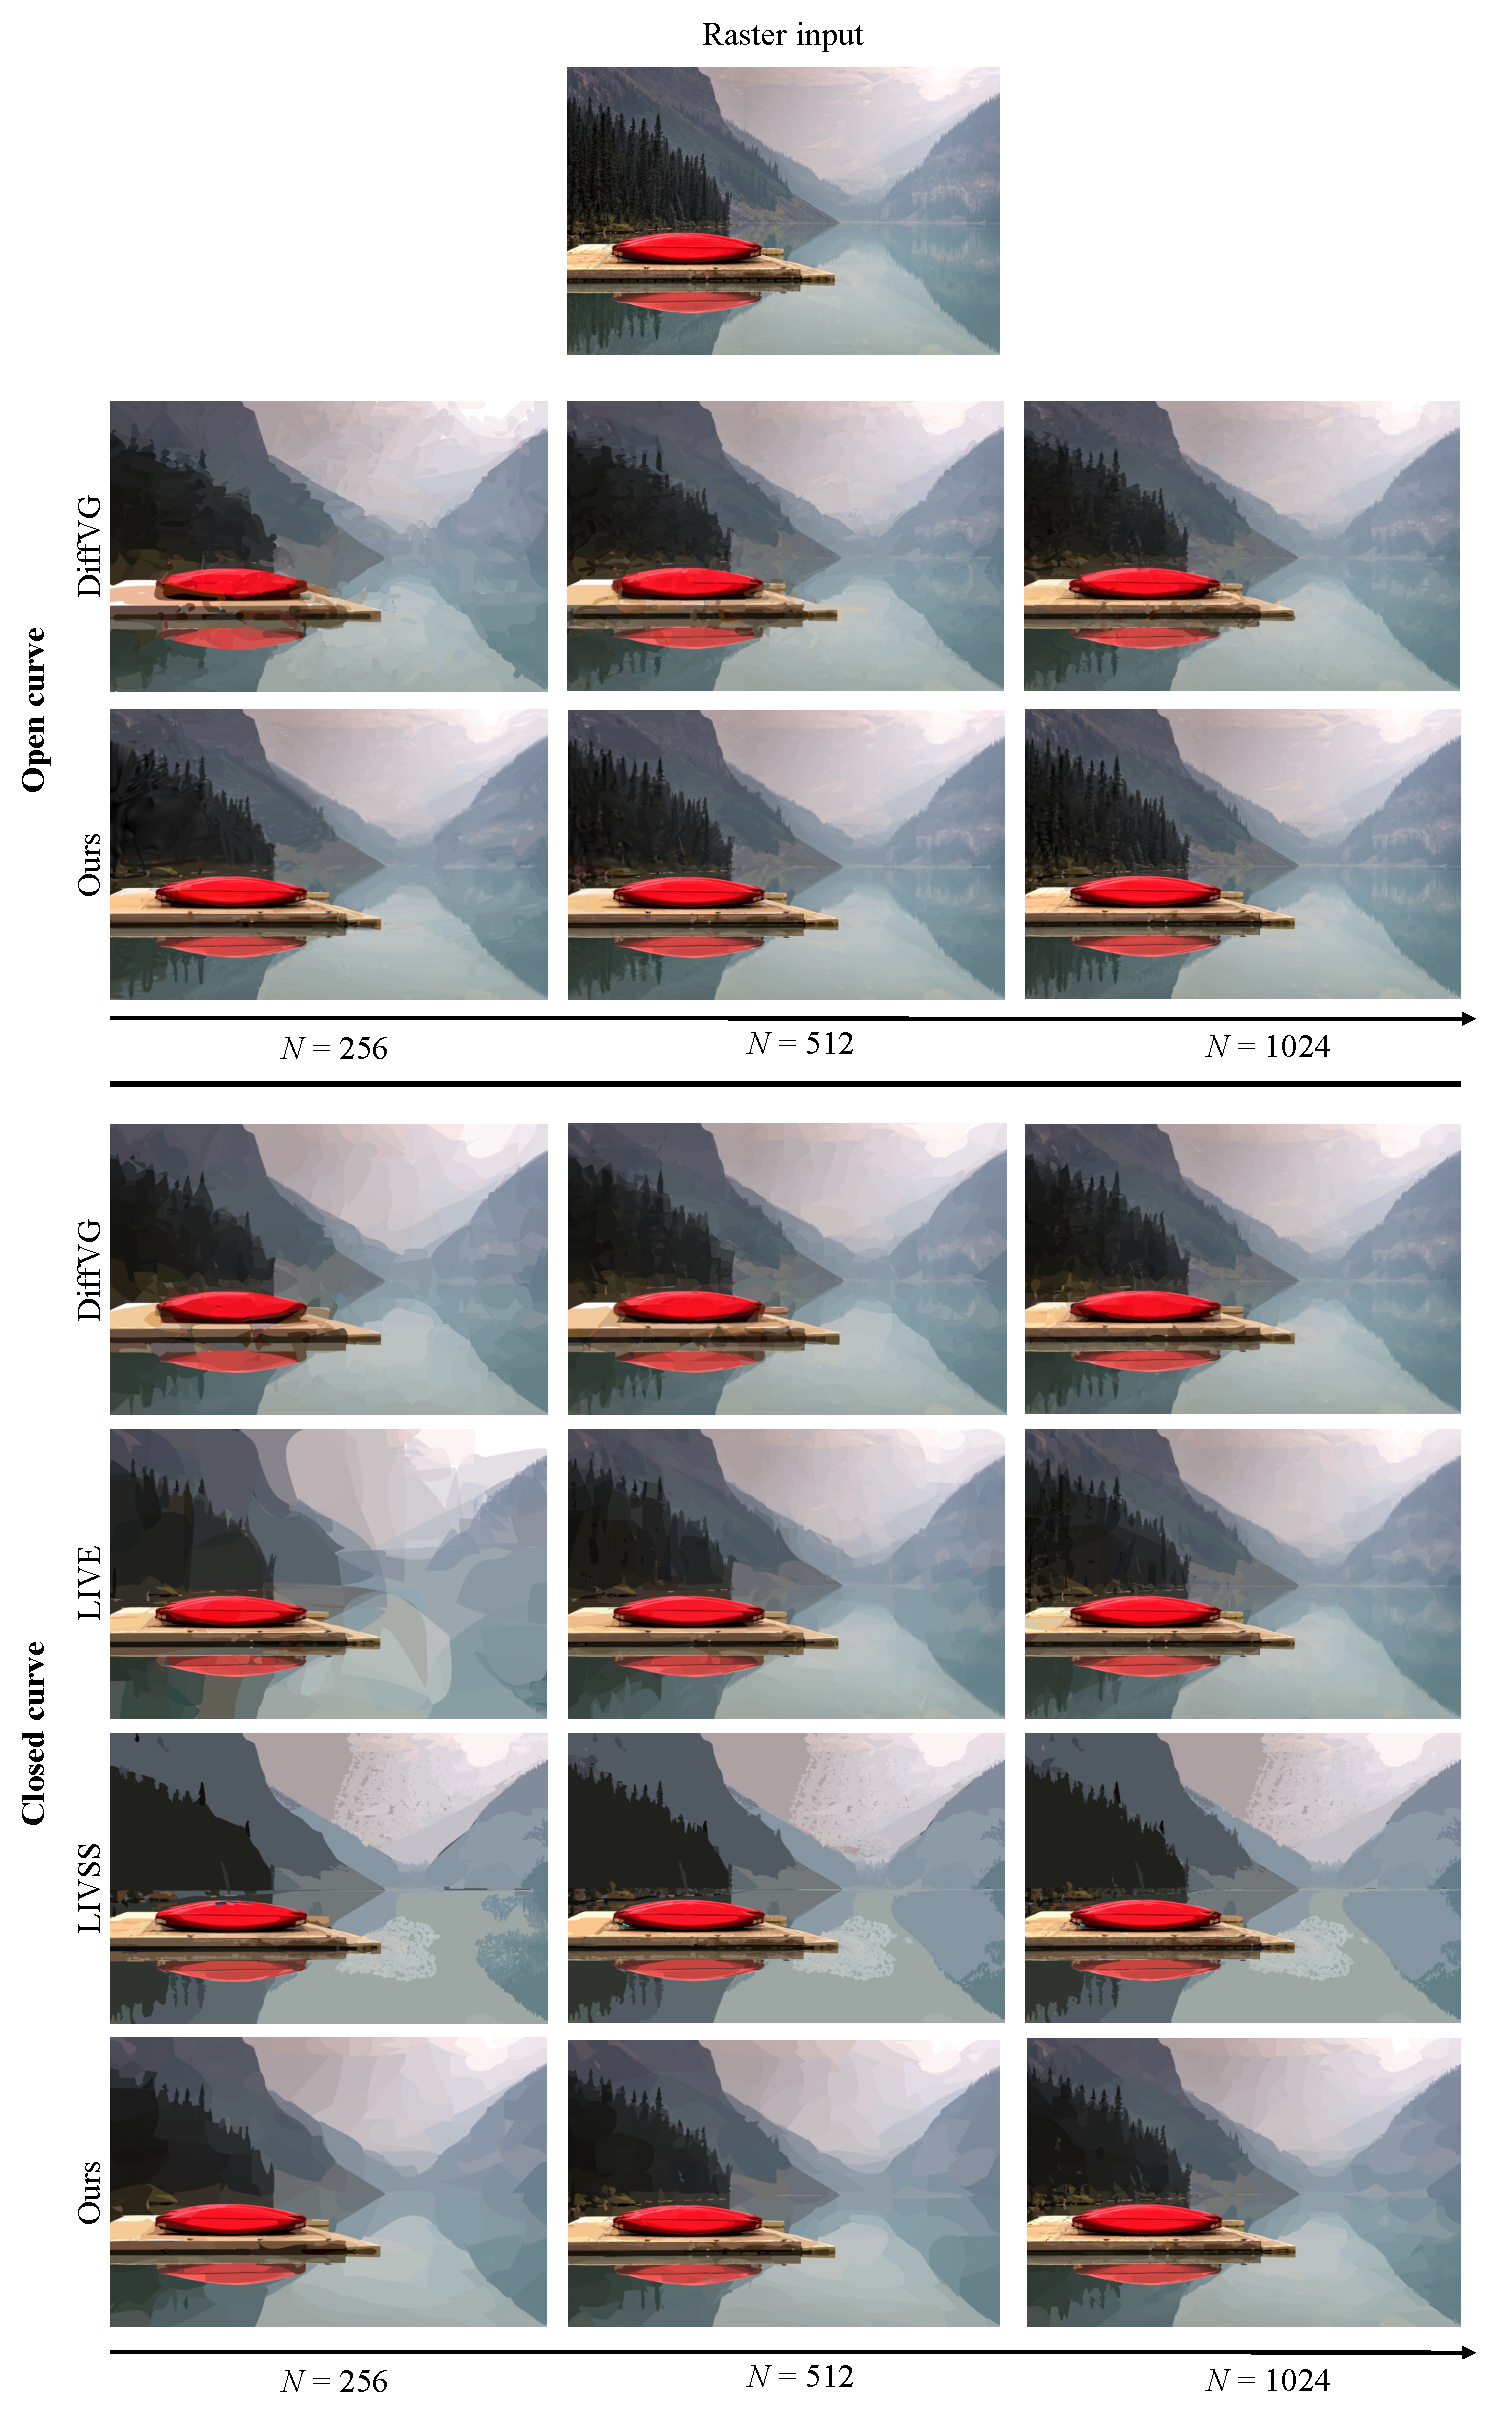
\includegraphics[width=1\linewidth]{figures/app_comparison_2.pdf}
% \vspace{-2em}
\caption{More qualitative comparisons of our method and the existing differentiable VG rasterization method on DIV2K dataset \cite{Timofte_2017_CVPR_Workshops}.
}
\label{fig:app_comparsion_2}
\end{figure*}

\begin{figure*}[t]
\centering
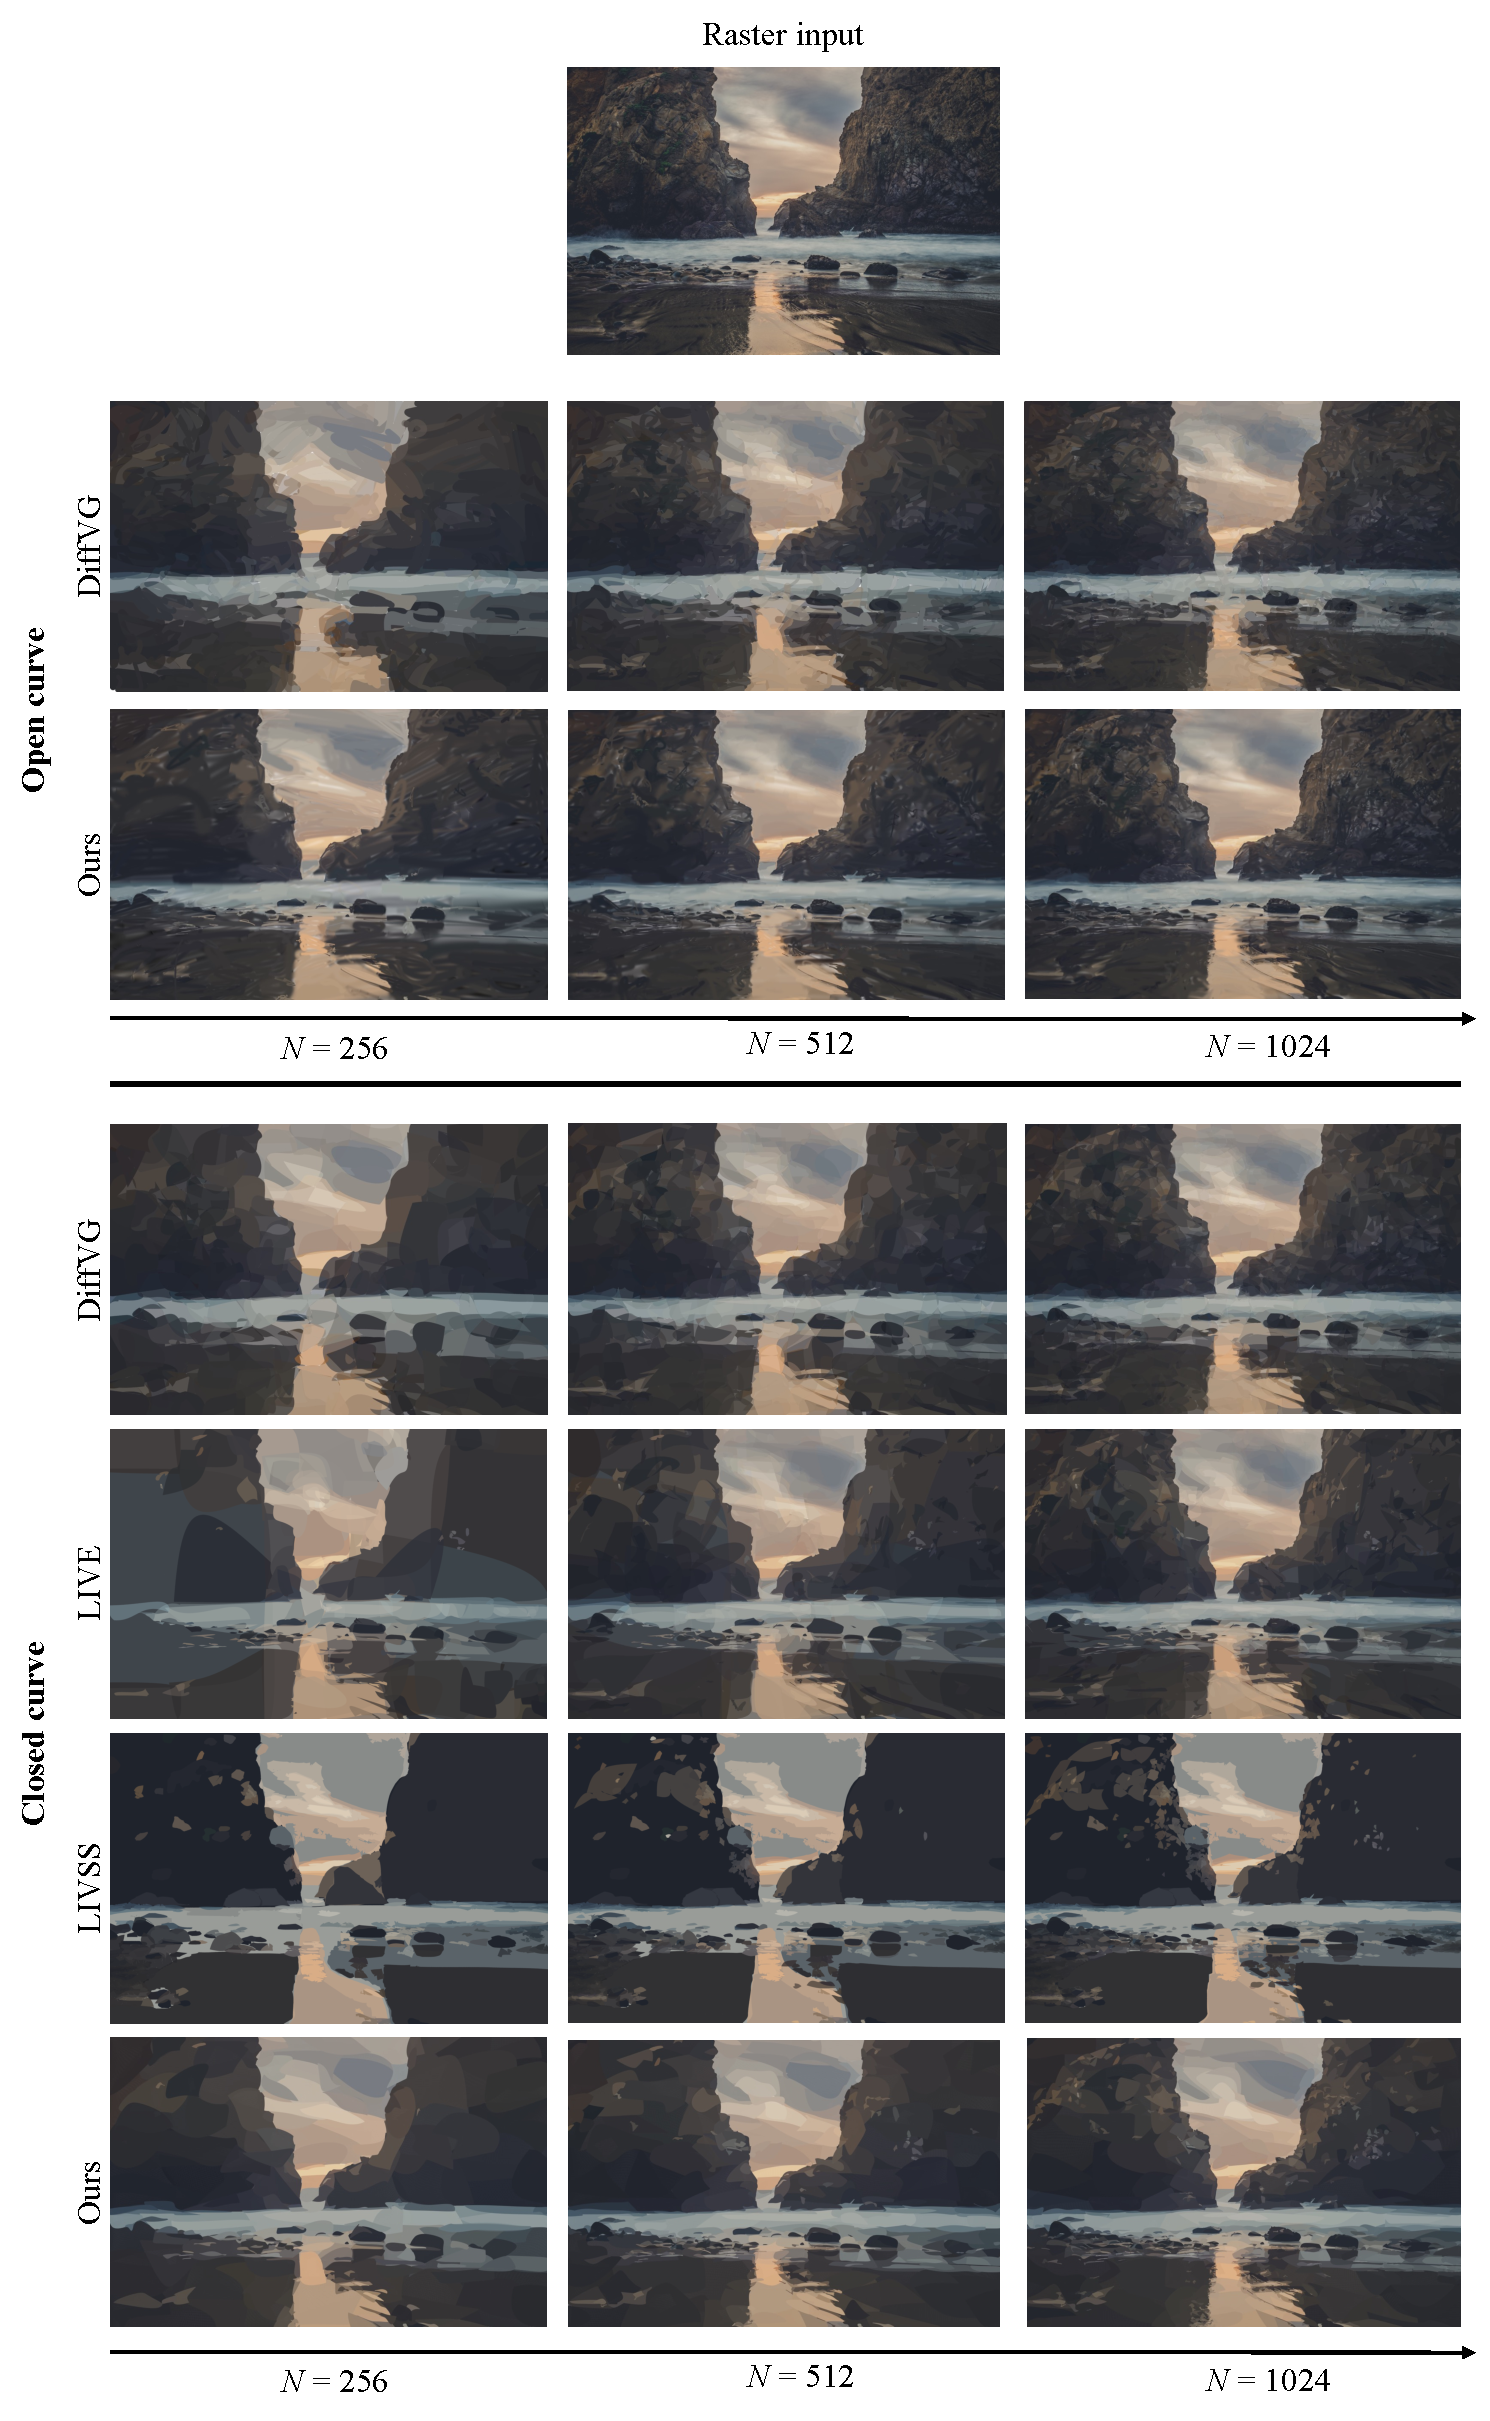
\includegraphics[width=1\linewidth]{figures/app_comparsion_3.pdf}
% \vspace{-2em}
\caption{More qualitative comparisons of our method and the existing differentiable VG rasterization method on DIV2K dataset \cite{Timofte_2017_CVPR_Workshops}.
}
\label{fig:app_comparsion_3}
\end{figure*}

\begin{figure*}[t]
\centering
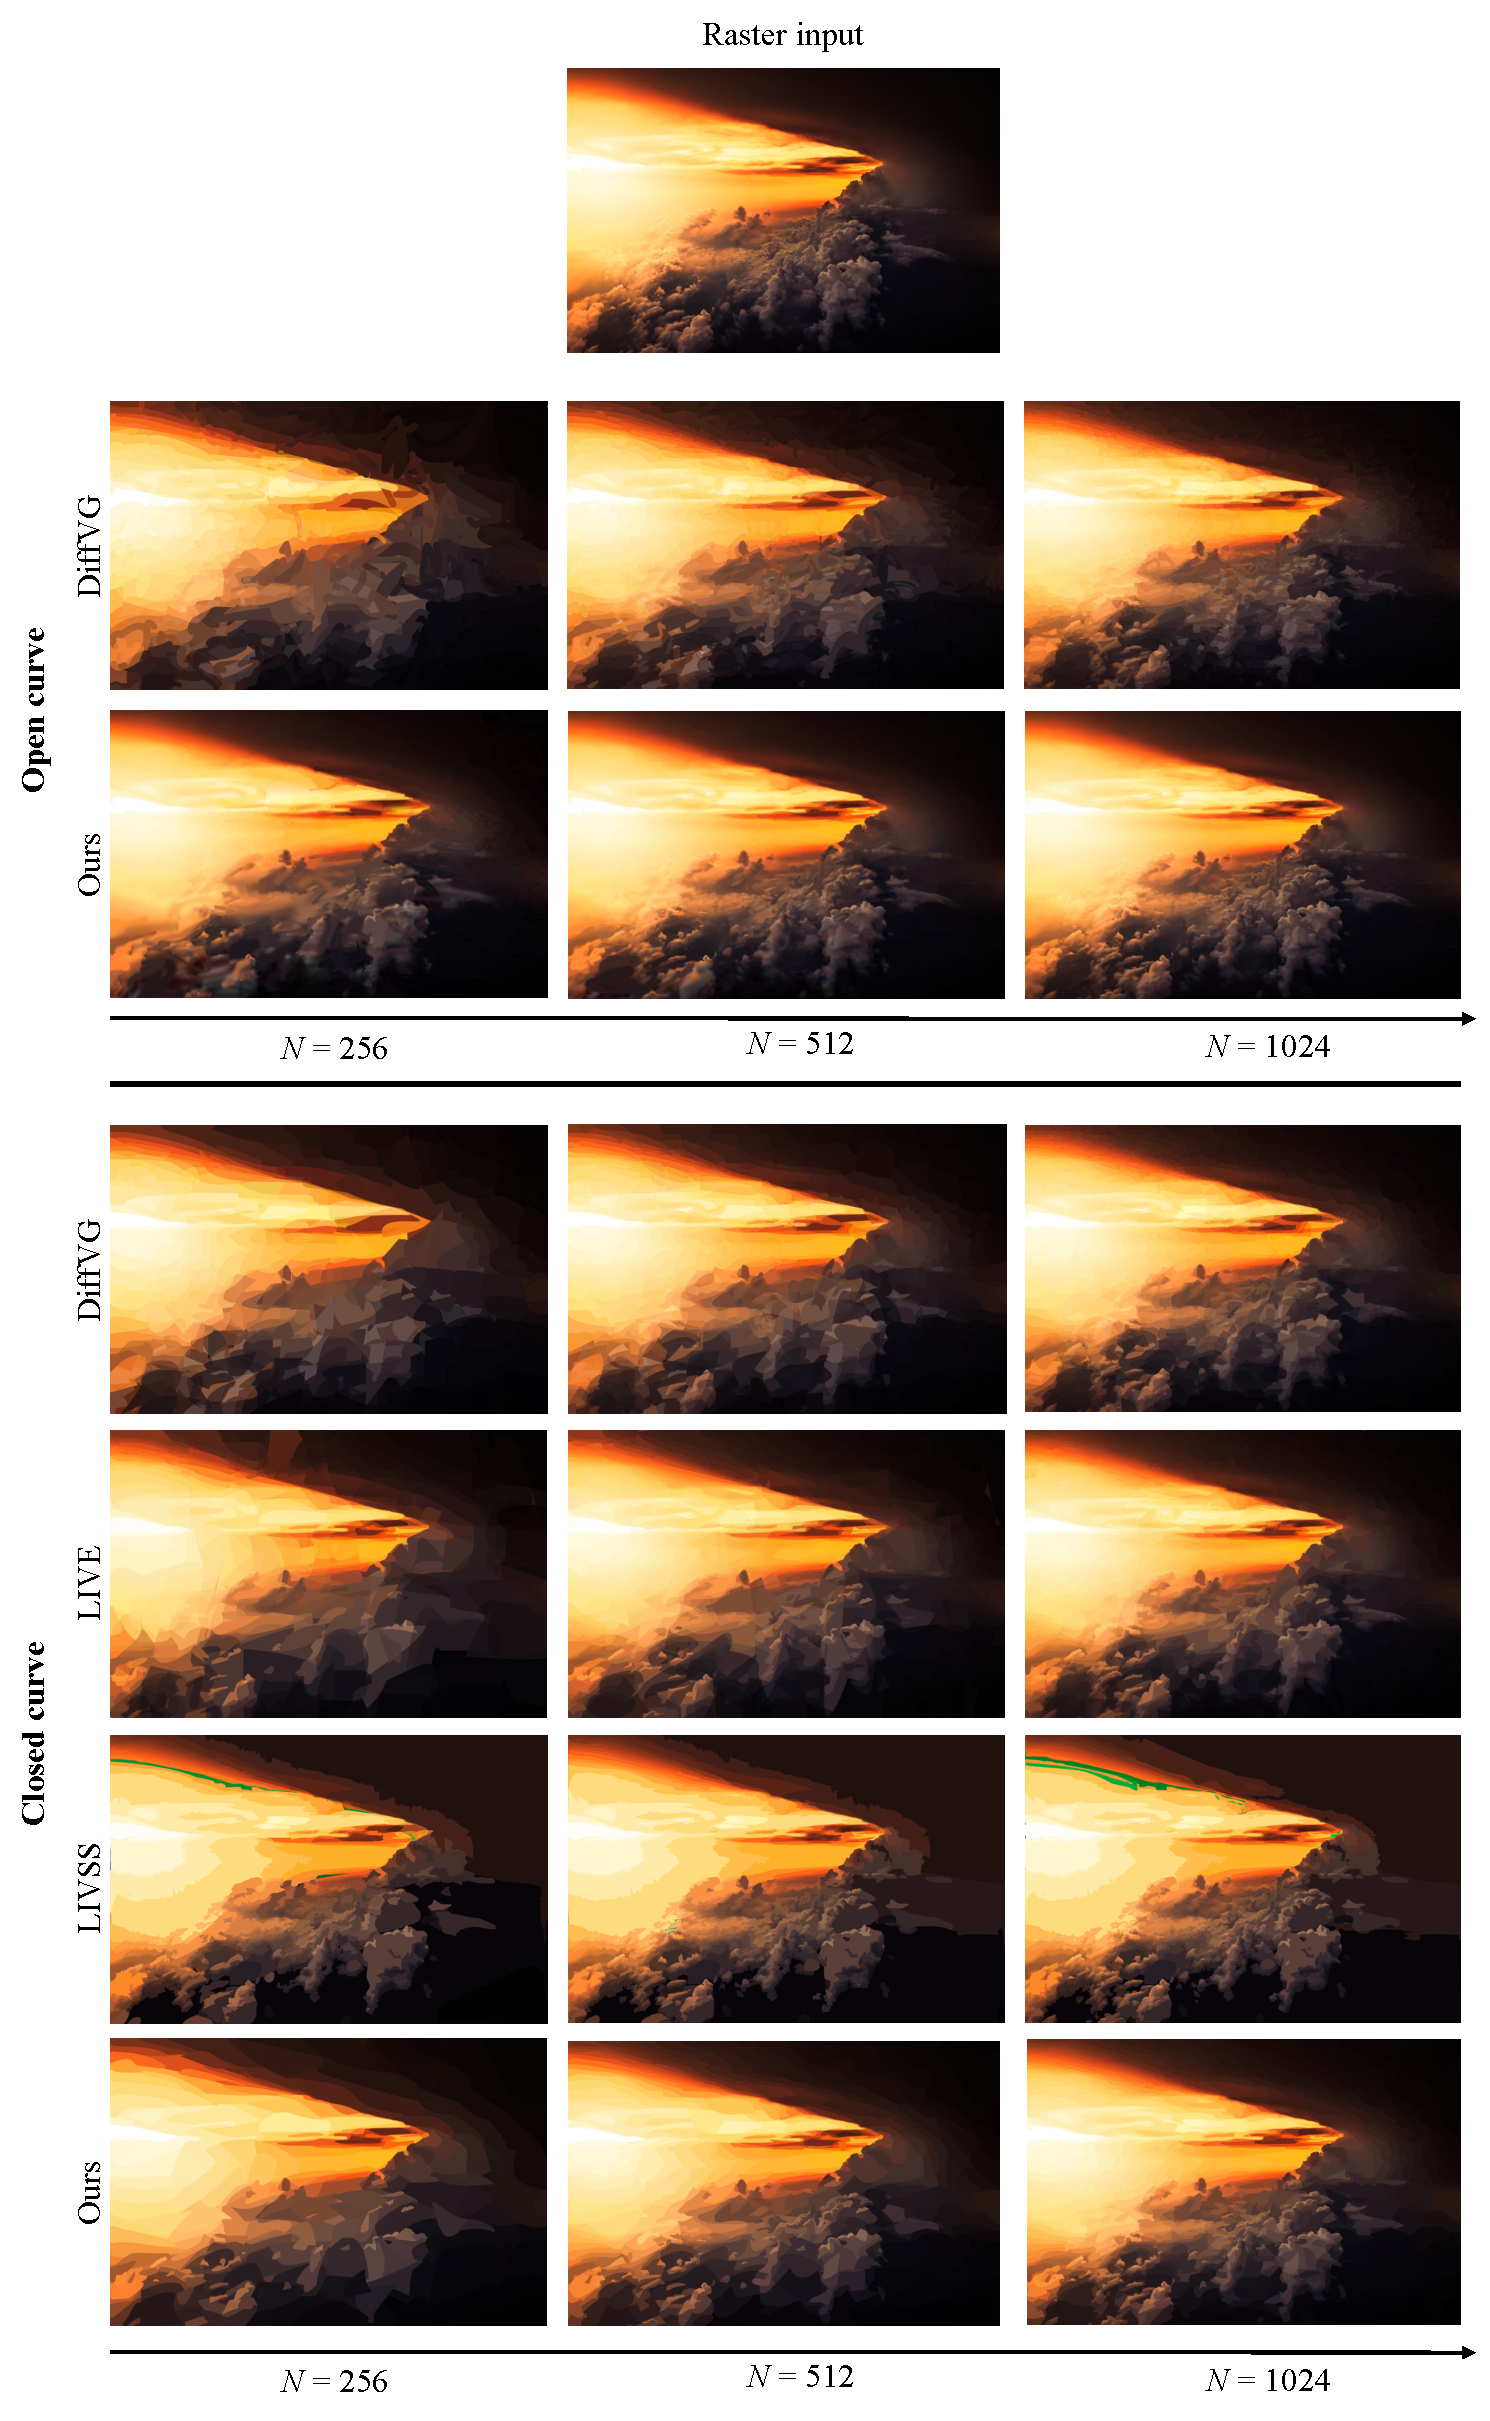
\includegraphics[width=1\linewidth]{figures/app_comparsion_4.pdf}
% \vspace{-2em}
\caption{More qualitative comparisons of our method and the existing differentiable VG rasterization method on DIV2K dataset \cite{Timofte_2017_CVPR_Workshops}.
}
\label{fig:app_comparsion_4}
\end{figure*}

\begin{figure*}[t]
\centering
\hspace*{-0.205\linewidth} 
\includegraphics[width=1.4\linewidth]{figures/More_DIV2K.pdf}
\caption{More image vectorization results by Bézier Splatting on DIV2K dataset \cite{Timofte_2017_CVPR_Workshops}.}
\label{fig:appendix_large_div}
\end{figure*}

\begin{figure*}[t]
\centering
\hspace*{-0.205\linewidth} 
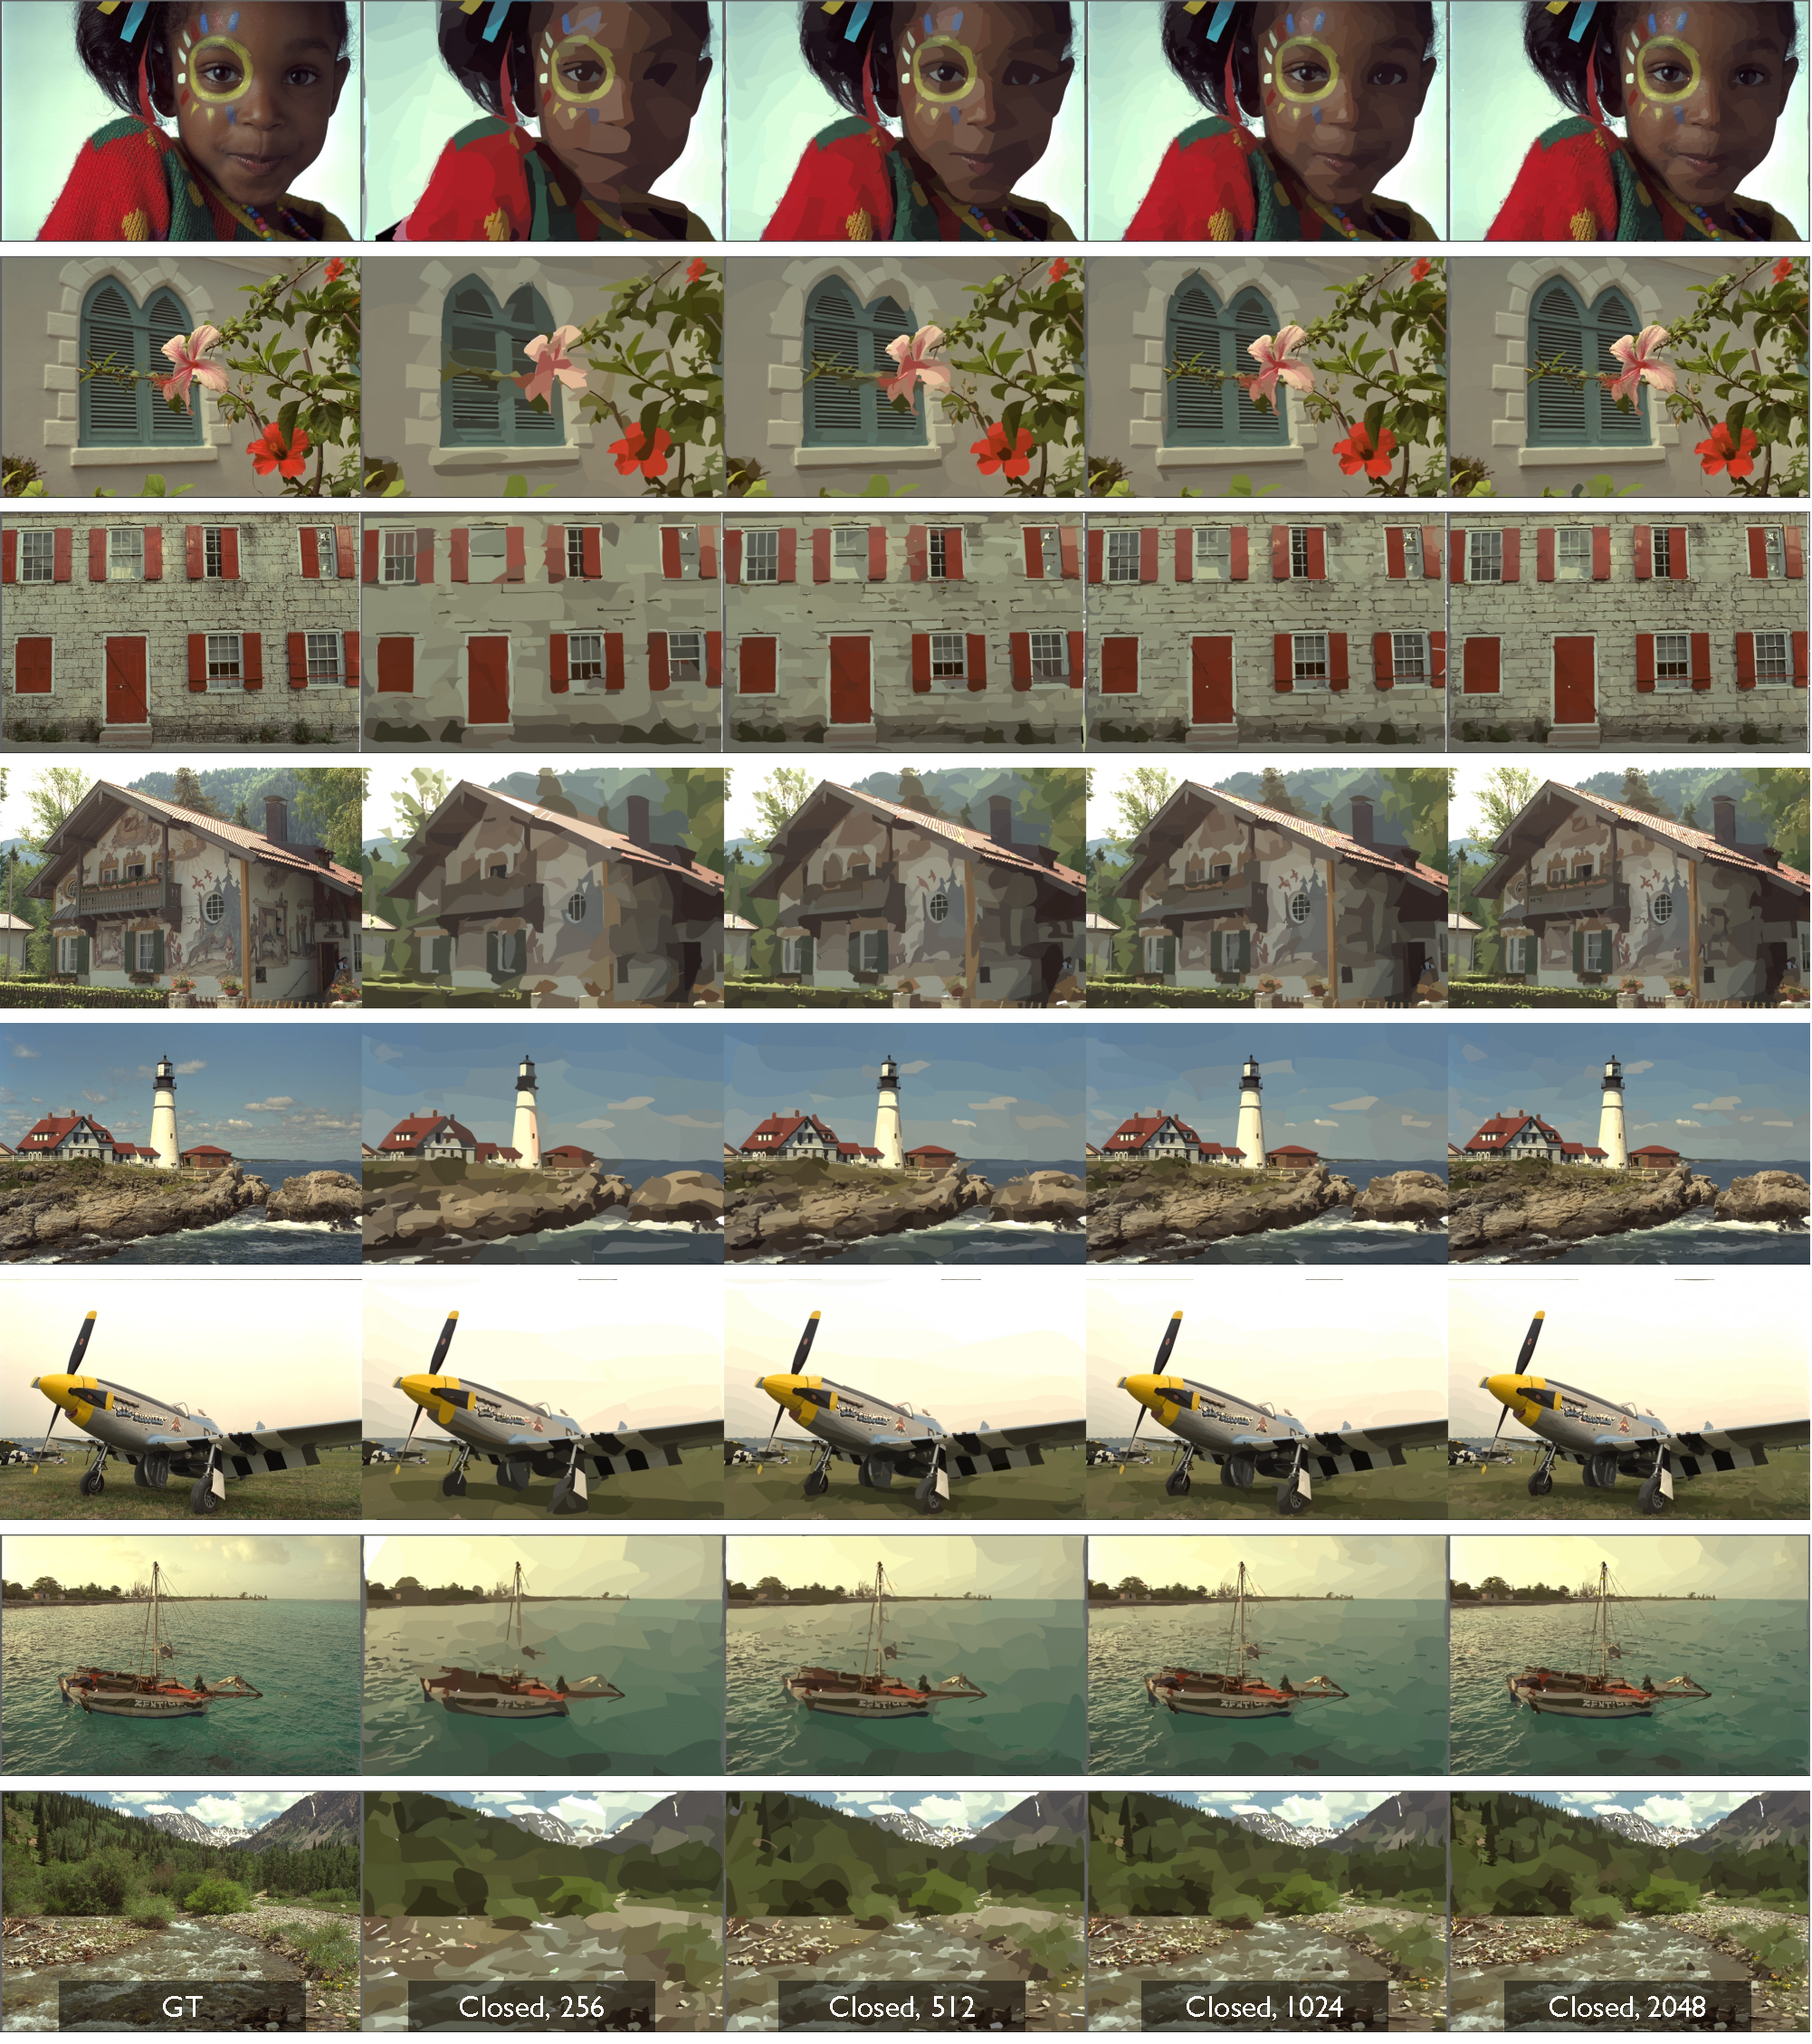
\includegraphics[width=1.4\linewidth]{figures/appendix_Kodak.pdf}
\caption{More image vectorization results by Bézier Splatting on Kodak \cite{kodak1999} dataset.}
\label{fig:appendix_Kodak}
\end{figure*}


% \begin{figure*}[t]
% \centering
% \includegraphics[width=1\linewidth]{figures/appendix_large_div_line.pdf}
% \caption{More image vectorization results by Bézier Splatting on DIV2K dataset \cite{Timofte_2017_CVPR_Workshops}.}
% \label{fig:appendix_large_line}
% \end{figure*}

% \begin{figure*}[t]
% \centering
% \includegraphics[width=1\linewidth]{figures/appendix_large_div_area.pdf}
% \caption{More image vectorization results by Bézier Splatting on DIV2K dataset \cite{Timofte_2017_CVPR_Workshops}.}
% \label{fig:appendix_large_closed}
% \end{figure*}

\begin{figure*}[t]
\centering
\hspace*{-0.205\linewidth} 
\includegraphics[width=1.4\linewidth]{figures/appendix_animation.pdf}
\caption{More image vectorization results by Bézier Splatting on DanbooRegion dataset \cite{DanbooRegion2020}.}
\label{fig:appendix_large_animation}
\end{figure*}

